% \label{chpt:results:evolutionary modelling} % for referencing this chapter elsewhere, use \ref{chpt:label}
% \lhead{\emph{Inferring mass loss rate from donor properties}} % This is for the header on each page - perhaps a shortened title

\label{chpt:Mass loss and Angular momentum loss in short period CVs} % for referencing this chapter elsewhere, use \ref{chpt:label}
\lhead{\emph{Mass loss and Angular momentum loss in short period CVs}} % This is for the header on each page - perhaps a shortened title

The structure of this chapter is as follows: first, I demonstrate that MESA is capable of reproducing the canonical CV donor tracks of \citet{knigge11}, and use MESA to evaluate the range of donor masses for which the method detailed in \S\ref{sect:modelling:evolutionary modelling} can be reasonably applied. I derive an empirical function for appropriate spot parameters as a function of donor mass, and use this to infer $\dot M_{\rm donor}$ and $\dot J$ for the well-characterised eclipse modelled CV sample.
Finally, I explore the implications of these data, and the correlations between them.

The analysis of this section includes eclipse modelled data from several sources: the 15 systems contained in this thesis, the 15 CVs characterised by \citet{McAllister2019}, and the 14 CVs modelled by \citet{Savoury2011}. An additional 4 systems from \citet{mcallister2015,mcallister2017, mcallister2017b}; and \citet{copperwheat2010} were used, detailed in Table~\ref{appendix:table:supplementary systems}. A full catalogue of all these data is given in Appendix~\ref{appendix:eclipse modelled CV data tables}.
There is some overlap between the data of \citet{McAllister2019} and \citet{Savoury2011}, and where this is the case the more recent findings of \citet{McAllister2019} are preferred.


\section{Reproducing the canonical CV donor tracks}
\label{sect:results:reproducing K11 tracks}

First, I demonstrate that MESA can closely reproduce the two \citet{knigge11} donor tracks -- recall from \S\ref{sect:introduction:the missing aml problem} that two such tracks are constructed, a `standard' track with only typical gravitational braking below the period gap, and an `optimal' track that amplifies gravitational braking by $2.47\times$.
By default, MESA shuts off magnetic braking when the donor becomes fully convective, a practice which I motivate in \S\ref{sect:introduction:the missing aml problem} to be spurious. Instead, MESA is altered for a fixed magnetic braking cutoff at $0.2 M_\odot$, arbitrarily fixing the donor mass of the period gap in line with \citet{knigge11}.

In addition, \citet{Pala2017a} added a subroutine to MESA that allows for the amplification of gravitational braking below the period gap.
This subroutine uses the \lstinline{s% other_jdot_mb} MESA hook, and simply scales the calculated gravitational braking by a user-defined parameter, though this was previously hard-coded in the subroutine and small changes were made to allow this scaling to be defined in the MESA configuration inlist.
This was used to reproduce the `optimal' track. The donor physics was configured as described in \S\ref{sect:modelling:MESA configs}, and the model is initialised with some additional binary configuration:
\begin{itemize}
    \item The two objects begin as $M_{\rm donor} = 0.65 M_\odot$, $M_{\rm wd} = 0.82$, at an orbital period of 12 hours.
    \item The white dwarf is not allowed to retain any accreted material,
    \begin{itemize}
        \item \lstinline{mass_transfer_beta = 1.0}, \lstinline{limit_retention_by_mdot_edd = .false.}
    \end{itemize}
    \item The white dwarf is considered as a point mass, with no evolution over time,
    \begin{itemize}
        \item \lstinline{evolve_both_stars = .false.}
    \end{itemize}
    \item The donor star has a fixed spot coverage fraction of $0.10$, chosen to match the period at which the donor emerges from the period gap.
\end{itemize}

These changes are enough to reproduce the \citet{knigge11} tracks to a reasonable degree; Figure~\ref{fig:results:MESA can reproduce the K11 tracks} shows the four model tracks in the short period regime.
Note that the small deviation at $\sim 0.13 M_\odot$ in the MESA models are due to MESA transitioning do a different equation of state, and is expected.
The small difference in gradient between the MESA models and the \citet{knigge11} models is due to the donor having a differing mass-radius relationship, as this model does not use variable star spot physics as the donor mass falls, described in \S\ref{sect:modelling:starspots in MESA} for reasons given in the next section.
With a more tailored donor configuration this could likely be improved without introducing the star spot physics at all, but this is not the focus of this study and the agreement is considered acceptable even with the suboptimal settings.

\begin{figure}
    \centering
    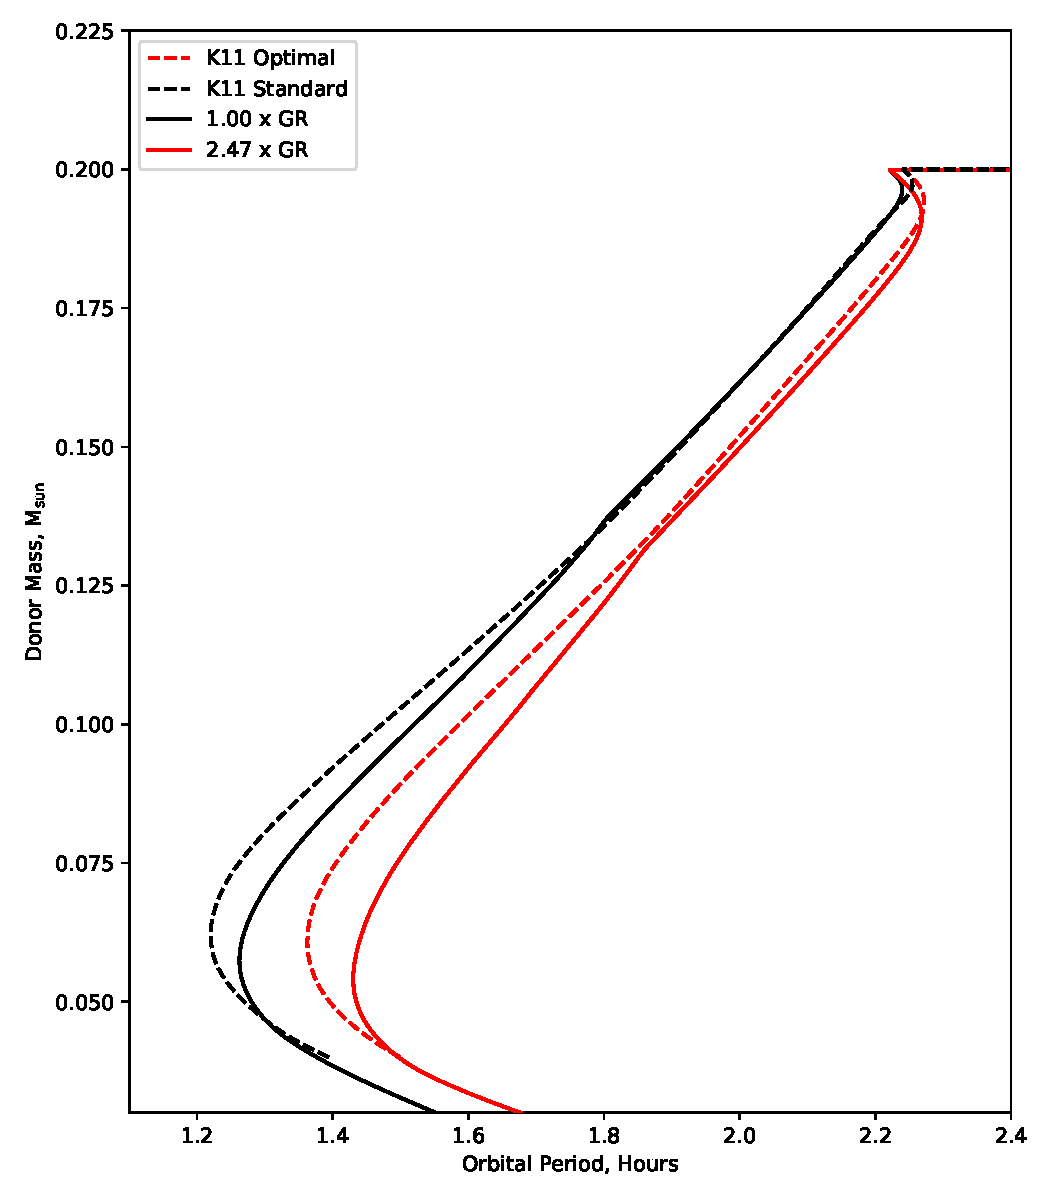
\includegraphics[width=.9\textwidth]{figures/modelling/reproducing_K11_tracks_fspot0.100.pdf}
    \caption{Showing how well MESA can reproduce the canonical \citet{knigge11} donor tracks. {\bf Solid lines} are MESA tracks, and {\bf dotted lines} are the \citet{knigge11} tracks. {\bf Black} lines have only gravitational braking below the period gap, and {\bf red} lines gave gravitational braking at $2.47\times$ strength. Here, MESA models have $f_{\rm spot} = 0.1$.}
    \label{fig:results:MESA can reproduce the K11 tracks}
\end{figure}



\section{For what range of masses can we extract mass loss rates?}
\label{sect:results:MESA massloss allowable mass range}

This section evaluates the feasibility of using the radius of a star to extract present-day mass loss rates.
The analysis of this section does not include any star spots, i.e. $f_{\rm spot} = 0$ for these models.
Recall from \S\ref{sect:introduction:period minimum and bouncers} the two timescales that govern the response of the donor to mass loss: $\tau_{\rm KH}$ and $\tau_{\dot M}$. These timescales are calculated by
\begin{align}
    \tau_{\rm KH} =& \frac{G M_{\rm donor}^2}{L_{\rm donor} R_{\rm donor}} \\[8pt]
    \tau_{\dot M} =& \frac{\dot M}{M_{\rm donor}}
\end{align}

If $\tau_{\rm KH} \ll \tau_{\dot M}$, the donor is able to maintain thermal equilibrium and is indistinguishable from a singleton star of the same mass.
If $\tau_{\rm KH} \gg \tau_{\dot M}$, the donor is \textit{not} able to maintain equilibrium, and mass loss is fast and adiabatic.
The donor is inflated by mass loss, but as the stellar structure reacts slowly to changes in mass loss, the movement of the structure towards equilibrium is interrupted by changes in mass loss rate. This makes the degree of inflation of the donor sensitive to the mass loss \textit{history} of the donor.
% The donor is inflated by mass loss, but because the stellar structure as a whole reacts relatively slowly, the effect of past mass loss is retained and the degree of inflation becomes sensitive to the mass loss \textit{history} of the donor.
However, calculating the two timescales for CVs reveals that for much of their lives, $\tau_{\rm KH} \sim \tau_{\dot M}$ \citep{knigge11} - meaning that most CV donors are \textit{almost} able to maintain thermal equilibrium, but are still mildly affected by mass loss.
Under this almost-equilibrium regime, mass loss induces some degree of radius inflation in the donor, but because the star adjusts on timescales comparable to $\tau_{\dot M}$, the degree of inflation only depends on the present-day average $\dot M$. In this regime, we can discard the mass loss history of the donor, and use the radius inflation as a diagnostic for the baseline mass loss rate.
% This is also the justification for the CV tracks in \S\ref{sect:results:reproducing K11 tracks} to not include the star spot radius correction. As the donor decreases in mass, the necessary spot parameters to correct its radius will change (refer to \S\ref{sect:modelling:tuning star spots to observations}). However, the donor structure would only react to a change in spot parameters on the $\tau_{\rm KH}$ timescale, causing a CV donor model to effectively have the `wrong' spot parameters for its mass, due to the time lag between parameters changing and the donor radius responding to that change.


Whether a donor radius is sensitive to its $\dot M$ history can be considered as a function of $M_{\rm donor}$. As $M_{\rm donor}$ falls, $\tau_{\rm KH}$ begins to rise faster than $\tau_{\dot M}$; Figure~\ref{fig:results:how does tauKH and tauMdot vary with donor mass} shows this trend, produced by a MESA model of a CV using the configuration provided in \citet{Paxton_2015}.
The rise in $\tau_{\rm KH}$ relative to $\tau_{\dot M}$ becomes significant at $\sim 0.1 M_\odot$, around the mass the donor enters the adiabatic $\tau_{\rm KH} \gg \tau_{\dot M}$ period bouncer phase c.f.~\S\ref{sect:introduction:period minimum and bouncers}.
\begin{figure}
    \centering
    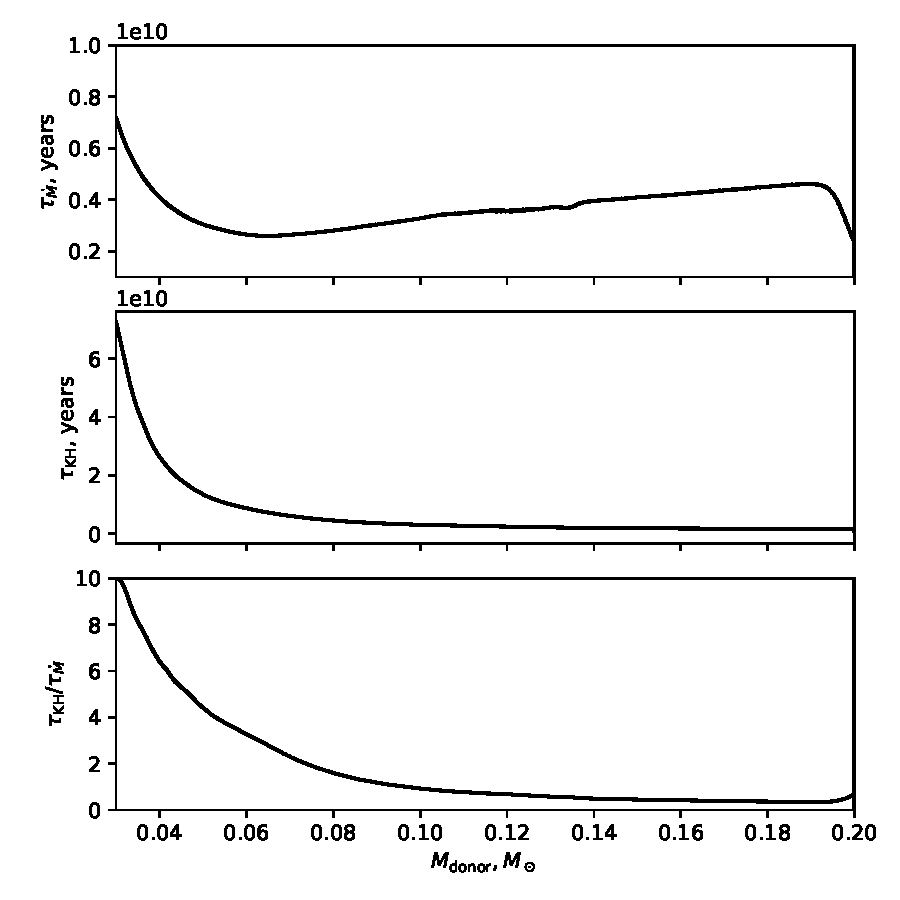
\includegraphics[width=\textwidth]{figures/modelling/tau_both_vs_donor_mass_AML000.pdf}
    \caption{Showing how the two timescales, $\tau_{\rm KH}$ and $\tau_{\dot M}$ vary with donor mass below the period gap in CV donors, as modelled by MESA \citep{Paxton_2015,Pala2017a}.}
    \label{fig:results:how does tauKH and tauMdot vary with donor mass}
\end{figure}

We can determine the range of donor masses for which $\tau_{\rm KH} \sim \tau_{\dot M}$ from MESA models.
First, a series of singleton models (using the MESA configuration given in \S\ref{sect:modelling:MESA configs}) were evaluated with varying amounts of fixed mass loss rates, uniformly spaced between $\log (\dot M, M_\odot \mathrm{yr}^{-1}) = -9.9 \rightarrow -10.8$.
Then, a series of MESA CV models were run with gravitational losses amplified by $x = 1 \rightarrow 6$, using the configuration and AML amplification in \S\ref{sect:results:reproducing K11 tracks}.
Finally, each model has its radius, $R$, and $\dot M$ extracted at $0.1 M_\odot$. Since the CV models have varying $\dot M$ and the singleton models do not, if $\dot M$ history does not affect radius inflation the radii between the two sets of models will match, and a disagreement indicates that history plays a significant role in radius inflation.
 Figure~\ref{fig:results:comparing radii at 0.1Msun} shows this, and little divergence between the two sets of radii is visible. However, note that higher $\dot M$ do show a small degree of divergence.
\begin{figure}
    \centering
    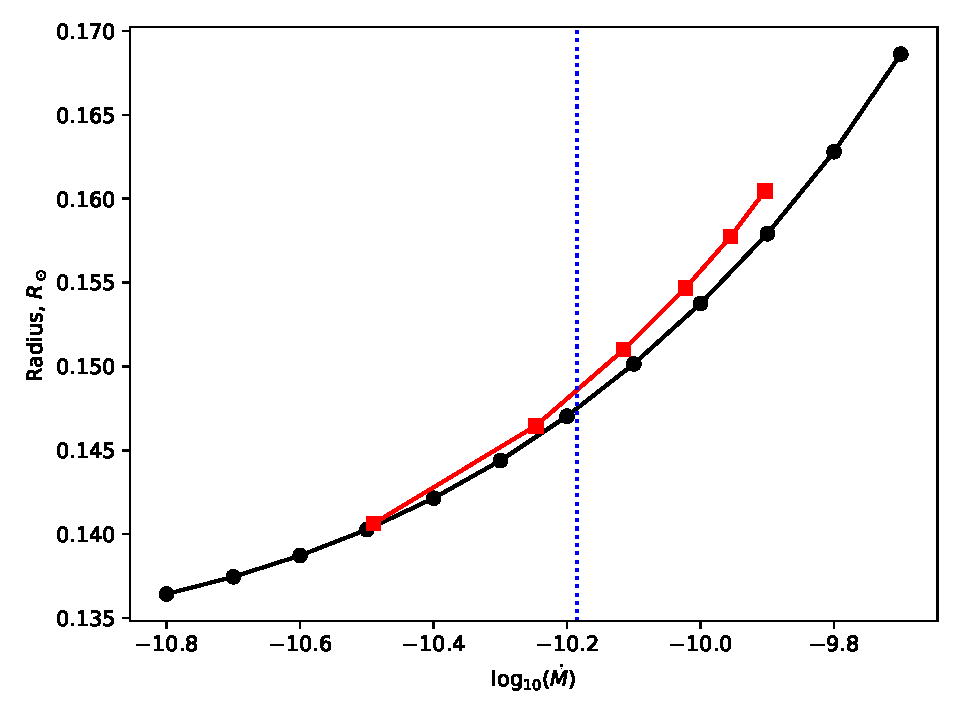
\includegraphics[width=.8\textwidth]{figures/modelling/compare_0.1Msun_with_CV_track_K11_fig1.pdf}
    \caption{Showing the radius and mass loss extracted from MESA models at $0.1 M_\odot$. The {\bf black} line is a series of singleton models with constant mass loss, and the {\bf red} line is a series of CV models with gravitational AML amplified by $x = 1 \rightarrow 6$, with the lowest $\dot M$ on the left. The {\bf blue dotted line} shows $\dot M$ for a CV with $2.47\times$ gravitational braking strength as predicted by a MESA CV model.}
    \label{fig:results:comparing radii at 0.1Msun}
\end{figure}

By plotting the difference between the two sets of models, and repeating the same process for a range of masses, Figure~\ref{fig:results:comparing radii over a range of masses} is produced. Now, by looking at what level of divergence historical changes in $\dot M$ induces at various donor masses, we can evaluate what mass range is acceptable. The upper limit on mass must be $0.2 M_\odot$, as this is the enforced mass of the period gap, and for a lower limit I impose an acceptable level of disagreement of $3\%$. It can be seen that the minimum acceptable mass is then $0.08 M_\odot$.
\begin{figure}
    \centering
    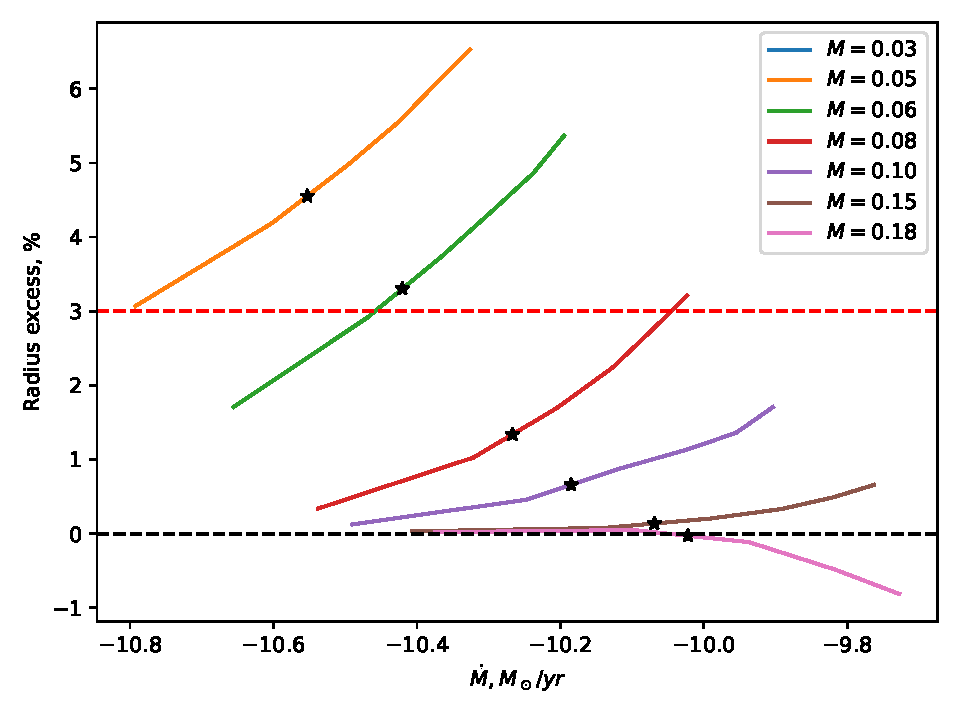
\includegraphics[width=\textwidth]{figures/modelling/compare_multiple_mass_with_CV_K11_fig1a.pdf}
    \caption{The inflation of CV model radii, $R_{CV}$ (whose $\dot M$ is time-dependent), over singleton model radii, $R_S$ (whose $\dot M$ is constant), from Figure~\ref{fig:results:comparing radii at 0.1Msun}, for a range of masses. The {\bf stars} on each line show the $\dot M$ and inflation for a model with gravitational braking at $2.47\times$ strength, mirroring the \citet{knigge11} optimal track. The {\bf red dashed line} shows the upper limit for acceptable disagreement, and the {\bf black dashed line} shows perfect agreement.}
    \label{fig:results:comparing radii over a range of masses}
\end{figure}



\section{Tuning star spot parameters to observations}
\label{sect:modelling:tuning star spots to observations}

With star spots implemented in MESA, the Brown relation can now be reproduced.
$x_{\rm spot}$ is fixed at 0 and $f_{\rm spot}$ is varied.
Since radius increases monotonically with $f_{\rm spot}$, a binary chop is performed (see \S\ref{sect:modelling:binary chop methodology}), optimising for $\Delta R=R_{\rm MESA}-(1.045\times R_{\rm Brown})=0$ at a stellar age of 2~Gyrs for a range of masses. The 4.5\% radius increase is to compensate for the non-spherical Roche geometry of the donor.
The resulting M-$f_{\rm spot}$ relation is shown in Figure~\ref{fig:modelling:fspot mass relationship}.

Below masses of $\sim 0.12 M_\odot$, the required $f_{\rm spot}$ becomes slightly negative, i.e. default MESA models are larger than observations plus the $4.5\%$ non-spherical correction.
Since a negative coverage fraction is unphysical, negative values of $f_{\rm spot}$ are set equal to 0, and it should be emphasised that derived mass loss rates may become somewhat unreliable below this mass.
Below $M_{\rm donor} = 0.121 M_\odot$ the brown relation transitions to the \citet{baraffe2015} theoretical tracks, so model agreement is perhaps unsurprising here. However, the clear trend in $f_{\rm spot}$ towards 0 prior to this suggests that the MESA radius calibration given here is still valid.
However, the severity of this unreliability is not catastrophic, as the minimum value of $f_{\rm spot}$ is still reasonably close to 0.

There is significant scatter in the Brown mass-radius relation, that is not captured in these models. The inherent scatter in radius for the observations is $\sim 3\%$ between 0.1 and 0.2 $M_\odot$, which adds to the uncertainty in modelled radius inflation, and thus mass loss rate.
Whilst this may skew an individual system, on average the inferred mass loss from model radius should be accurate. Therefore, this effect should not skew the $\dot M$ results with a large enough sample size.

\begin{figure}
    \centering
    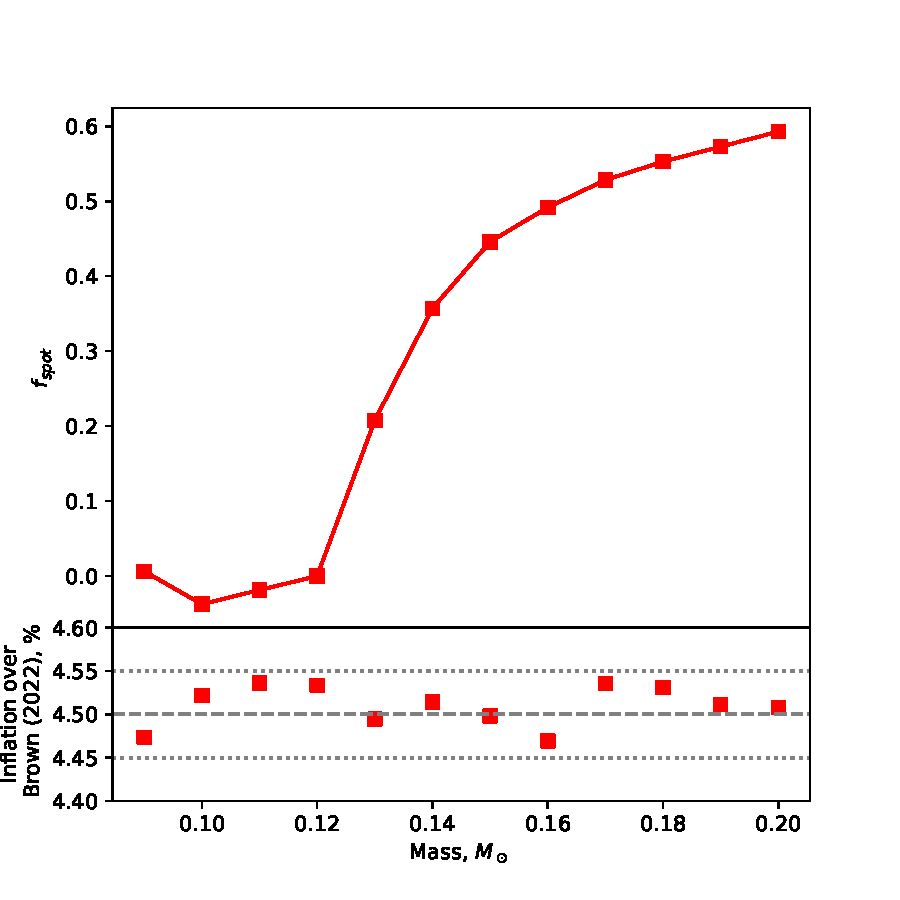
\includegraphics[width=\textwidth]{figures/modelling/fspot_relation_to_match_brown_plus_4.5.pdf}
    \caption{{\it Top}: The required $f_{\rm spot}$ that is applied to tune M dwarf MESA models to match the Brown relation, plus an added $4.5\%$ inflation due to non-spherical Roche geometry. {\it Bottom}: the residuals from the best fit value of $f_{\rm spot}$. The {\bf dotted lines} show the acceptable deviation from perfect agreement in order to terminate the binary chop, and the {\bf dashed line} shows the target inflation. Note that when finding the necessary value of $f_{\rm spot}$ to match the Brown relation $x_{\rm spot} \equiv 0$, and negative values of $f_{\rm spot}$ were allowed. However, in all subsequent modelling, negative $f_{\rm spot}$ were set to 0. {\bf Red squares} show evaluated MESA models.}
    \label{fig:modelling:fspot mass relationship}
\end{figure}



\section{Inferred mass loss rates of CV donors}
\label{sect:modelling:donor mass loss rates}

Overall, there are 34 systems with eclipse-modelled characterisations available with donors in the correct mass range of $0.08 M_\odot < M_{\rm donor} < 0.20 M_\odot$, catalogued in Table~\ref{table:results:mdot modelling}.
The special case of SDSS J1524 is included despite having a donor mass of $0.074\pm0.008$, slightly below $0.08 M_\odot$, as the measurement is within $1\sigma$ of this limit.
% The properties of these donors, and their inferred $\dot M$, is given in Table~\ref{table:results:mdot modelling}.

% {\bf The reported central values were optimised with a binary chop algorithm, but uncertainties were characterised by interpolation. This is considered a valid uncertainty, as the interpolation produced a central value within $1\sigma$ of the binary chop value in all cases.
% Note that there was a single exception to this; in the case of ASASN-17fo, whilst the interpolator was unable to find an appropriate $\dot M$, the binary chop approach converged on a reasonable value of $\log (\dot M,\ M_{\odot}\ {\rm yr}^{-1} = -10.86$. This leaves this value with no characterised error, so an arbitrary error of $\pm 0.5$ dex was used during later analysis.}
% {\it\bf The reported central values were optimised using a binary chop algorithm. To find the uncertainty in $\dot M$, two further combinations of donor mass and radius were evaluated for each system: ($M = \bar M + \sigma_M$, $R = \bar R + \sigma_R$), and ($M = \bar M - \sigma_M$, $R = \bar R - \sigma_R$). The donor mass and radius are highly correlated (typical cross-correlation coefficient values for the eclipse modelled systems analysed for this work are $\sim 0.9995$), so this is reasonable approximation to make.
% }

Note that not all systems in Table~\ref{table:results:mdot modelling} are assigned a $\dot M$.
This is due some donors being smaller than the Brown relation adjusted for non-spherical geometry, resulting in negative inflation that cannot be achieved by the introduction of mass loss.
Ideally, the inflation of a donor would be marginalised over the scatter of the observed M dwarf population about the Brown relation, which would likely solve this issue.
However, the population of M dwarfs becomes extremely sparse below $0.121 M_\odot$, and switches to the \citet{baraffe2015} theoretical models.
Attempting to characterise the scatter of these data is premature, though Gaia DR3 may introduce enough data to enable this in the near future.

Table~\ref{table:results:Jdot results} shows the AML rates calculated using Equation~\ref{eqn:modelling:Jdot from Mdot} for the systems for which $\dot M$ could be calculated from donor properties. Also shown is the AML expected from gravitational losses alone for that system, and the ratio between the observed and expected values.

\begin{table*}
    \centering
    \caption{The inferred $\dot M$ for eclipse-modelled CVs. For the Source column, `W22' are from Chapter~\ref{chpt:results:characterisation of 12 new CVs}, `M19' are systems modelled by \citet{McAllister2019}, `M17b' is from \citet{mcallister2017b}, `S11' are from \citet{Savoury2011}}
    \label{table:results:mdot modelling}
    \begin{tabular}{llccc}
        \hline \\
        {\bf System Name:} & \textbf{Source} & \textbf{$M_{\rm donor}, M_\odot$}  & \textbf{$R_{\rm donor}, R_\odot$}  & \textbf{$\log_{10}(\dot M,\ M_\odot / {\rm yr})$} \\
        \hline \hline \\
        ASASSN-14hq         &  W22      & $0.097 \pm 0.002$ & $0.157 \pm 0.001$ & $ -9.897 \pm 0.008$ \\
        ASASSN-15pb         &  W22      & $0.148 \pm 0.008$ & $0.209 \pm 0.003$ & $ -9.997 \pm 0.164$ \\
        ASASSN-17fo         &  W22      & $0.109 \pm 0.001$ & $0.144 \pm 0.001$ & $-10.859 \pm 0.137$ \\
        AY For              &  W22      & $0.106 \pm 0.005$ & $0.162 \pm 0.002$ & $ -9.918 \pm 0.024$ \\
        CSS090419           &  W22      & $0.087 \pm 0.016$ & $0.152 \pm 0.006$ & $ -9.859 \pm 0.003$ \\
        CSS090622           &  W22      & $0.105 \pm 0.009$ & $0.155 \pm 0.004$ & $-10.046 \pm 0.074$ \\
        MASTER OT J0014     &  W22      & $0.123 \pm 0.006$ & $0.165 \pm 0.002$ & $-10.279 \pm 0.328$ \\
        OGLE82              &  W22      & $0.132 \pm 0.003$ & $0.170 \pm 0.001$ & $-11.686 \pm 1.078$ \\
        SDSS J0748          &  W22      & $0.085 \pm 0.010$ & $0.128 \pm 0.005$ & $-10.438 \pm 0.152$ \\
        SDSS J1524          &  W22      & $0.074 \pm 0.007$ & $0.132 \pm 0.004$ & $-10.111 \pm 0.000$ \\
        CSS080623           &  M19      & $0.081 \pm 0.005$ & $0.128 \pm 0.002$ & $-10.343 \pm 0.041$ \\
        CSS110113           &  M19      & $0.105 \pm 0.007$ & $0.149 \pm 0.003$ & $-10.272 \pm 0.129$ \\
        OY Car              &  M19      & $0.093 \pm 0.004$ & $0.139 \pm 0.001$ & $-10.278 \pm 0.046$ \\
        SDSS J0901          &  M19      & $0.138 \pm 0.007$ & $0.182 \pm 0.003$ & $-10.547 \pm 0.368$ \\
        SDSS J1152          &  M19      & $0.094 \pm 0.016$ & $0.147 \pm 0.006$ & $-10.062 \pm 0.156$ \\
        SSS100615           &  M19      & $0.083 \pm 0.005$ & $0.128 \pm 0.002$ & $-10.384 \pm 0.038$ \\
        ASASSN-14ag         &  M17b     & $0.093 \pm 0.010$ & $0.135 \pm 0.007$ & $-10.416 \pm 0.211$ \\
        CTCV J2354-4700     &  S11      & $0.101 \pm 0.003$ & $0.146 \pm 0.001$ & $-10.245 \pm 0.030$ \\
        SDSS J1152          &  S11      & $0.087 \pm 0.006$ & $0.142 \pm 0.003$ & $-10.068 \pm 0.025$ \\
        OU Vir              &  S11      & $0.116 \pm 0.002$ & $0.163 \pm 0.001$ & $-10.067 \pm 0.026$ \\
        XZ Eri              &  S11      & $0.091 \pm 0.004$ & $0.135 \pm 0.001$ & $-10.352 \pm 0.054$ \\
        SDSS J0903          &  S11      & $0.099 \pm 0.004$ & $0.136 \pm 0.002$ & $-10.677 \pm 0.155$ \\
        SDSS J1227          &  S11      & $0.089 \pm 0.002$ & $0.137 \pm 0.001$ & $-10.243 \pm 0.017$ \\
        SDSS J1502          &  S11      & $0.078 \pm 0.001$ & $0.124 \pm 0.001$ & $-10.377 \pm 0.008$ \\
        ASASSN-14kb         &  W22      & $0.134 \pm 0.003$ & $0.164 \pm 0.001$ & -                   \\
        CTCV 1300-3052      &  M19      & $0.166 \pm 0.006$ & $0.211 \pm 0.002$ & -                   \\
        DV UMa              &  M19      & $0.187 \pm 0.012$ & $0.215 \pm 0.005$ & -                   \\
        IY UMa              &  M19      & $0.141 \pm 0.007$ & $0.177 \pm 0.002$ & -                   \\
        SSS130413           &  M19      & $0.140 \pm 0.012$ & $0.163 \pm 0.004$ & -                   \\
        V713 Cep            &  M19      & $0.176 \pm 0.018$ & $0.208 \pm 0.005$ & -                   \\
        Z Cha               &  M19      & $0.152 \pm 0.005$ & $0.182 \pm 0.002$ & -                   \\
        CTCV J1300-3052     &  S11      & $0.177 \pm 0.021$ & $0.215 \pm 0.008$ & -                   \\
        DV UMa              &  S11      & $0.196 \pm 0.005$ & $0.218 \pm 0.001$ & -                   \\
        % CSS090102           &  W22      & $0.059 \pm 0.003$ & $0.119 \pm 0.002$ & $-10.255 \pm 0.024$ \\
        % ASASSN-16kr         &  W20      & $0.042 \pm 0.003$ & $0.106 \pm 0.002$ & $-10.672 \pm 0.274$ \\
        % SSSJ1502-3505       &  W20      & $0.042 \pm 0.003$ & $0.106 \pm 0.003$ & $-10.648 \pm 0.206$ \\
        % SDSS 1501           &  M19      & $0.061 \pm 0.004$ & $0.113 \pm 0.002$ & $-10.456 \pm 0.034$ \\
        % SDSS J1057+2759     &  M17a     & $0.044 \pm 0.002$ & $0.109 \pm 0.001$ & $-10.514 \pm 0.102$ \\
        % PHL 1445            &  M15      & $0.064 \pm 0.005$ & $0.109 \pm 0.004$ & $-10.660 \pm 0.101$ \\
        % SDSS 1035           &  S11      & $0.048 \pm 0.001$ & $0.105 \pm 0.001$ & $-10.742 \pm 0.011$ \\
        % SDSS J1501          &  S11      & $0.077 \pm 0.010$ & $0.122 \pm 0.005$ & $-10.429 \pm 0.066$ \\
        % ASASSN-17jf         &  W20      & $0.060 \pm 0.008$ & $0.112 \pm 0.004$ & -                   \\
        % GY Cnc              &  M19      & $0.394 \pm 0.022$ & $0.446 \pm 0.009$ & -                   \\
        % SDSS 1006           &  M19      & $0.370 \pm 0.060$ & $0.457 \pm 0.026$ & -                   \\
        % SDSS 1702           &  S11      & $0.223 \pm 0.010$ & $0.252 \pm 0.004$ & -                   \\
        % SDSS 1507           &  S11      & $0.058 \pm 0.002$ & $0.097 \pm 0.001$ & -                   \\
        % SDSS 1433           &  S11      & $0.057 \pm 0.001$ & $0.107 \pm 0.001$ & -                   \\
        % IP Peg              &  C10      & $0.550 \pm 0.020$ & $0.466 \pm 0.006$ & -                   \\
        \hline
    \end{tabular}
\end{table*}

\begin{table*}
    \centering
    \caption{The inferred AML rates for the CVs in this sample. $\dot J_{\rm total}$ is calculated from the inferred $\dot M$, and $\dot J_{\rm GR}$ is the calculated gravitational AML rate. Sources are keyed the same as Table~\ref{table:results:mdot modelling}.}
    \label{table:results:Jdot results}
    \begin{tabular}{llccc}
        \hline
        {\bf System Name:} & \textbf{Source}  & \textbf{$\log(\dot J_{\rm total}, J)$} & \textbf{$\log(\dot J_{\rm GR}, J)$} & \textbf{$\dot J_{\rm total} / \dot J_{\rm GR}$} \\
        \hline \hline
        ASASSN-14hq     &  W22      & $27.157 \pm 0.009$    & $26.681 \pm 0.007$    & $2.996 \pm 0.081$ \\
        ASASSN-15pb     &  W22      & $27.091 \pm 0.162$    & $26.796 \pm 0.013$    & $2.115 \pm 0.818$ \\
        ASASSN-17fo     &  W22      & $26.240 \pm 0.137$    & $26.711 \pm 0.004$    & $0.355 \pm 0.114$ \\
        AY For          &  W22      & $27.184 \pm 0.026$    & $26.705 \pm 0.015$    & $3.021 \pm 0.204$ \\
        CSS090419       &  W22      & $27.158 \pm 0.039$    & $26.634 \pm 0.058$    & $3.381 \pm 0.548$ \\
        CSS090622       &  W22      & $26.994 \pm 0.078$    & $26.699 \pm 0.028$    & $2.011 \pm 0.388$ \\
        MASTER OT J0014 &  W22      & $26.842 \pm 0.325$    & $26.745 \pm 0.014$    & $1.661 \pm 1.488$ \\
        OGLE82          &  W22      & $25.428 \pm 1.083$    & $26.767 \pm 0.009$    & $0.980 \pm 8.280$ \\
        SDSS J0748      &  W22      & $26.645 \pm 0.156$    & $26.629 \pm 0.053$    & $1.116 \pm 0.442$ \\
        SDSS J1524      &  W22      & $26.990 \pm 0.015$    & $26.568 \pm 0.061$    & $2.672 \pm 0.390$ \\
        CSS080623       &  M19      & $26.705 \pm 0.042$    & $26.615 \pm 0.026$    & $1.238 \pm 0.141$ \\
        CSS110113       &  M19      & $26.895 \pm 0.128$    & $26.701 \pm 0.019$    & $1.633 \pm 0.502$ \\
        OY Car          &  M19      & $26.844 \pm 0.046$    & $26.666 \pm 0.014$    & $1.517 \pm 0.168$ \\
        SDSS J0901      &  M19      & $26.536 \pm 0.368$    & $26.780 \pm 0.014$    & $0.815 \pm 0.870$ \\
        SDSS J1152      &  M19      & $26.954 \pm 0.157$    & $26.656 \pm 0.073$    & $2.149 \pm 0.894$ \\
        SSS100615       &  M19      & $26.730 \pm 0.039$    & $26.625 \pm 0.024$    & $1.282 \pm 0.138$ \\
        ASASSN-14ag     &  M17b     & $26.587 \pm 0.215$    & $26.657 \pm 0.056$    & $0.968 \pm 0.526$ \\
        CTCV J2354-4700 &  S11      & $26.899 \pm 0.032$    & $26.691 \pm 0.008$    & $1.616 \pm 0.122$ \\
        % SDSS J1152      &  S11      & $26.917 \pm 0.030$    & $26.642 \pm 0.026$    & $1.893 \pm 0.172$ \\
        OU Vir          &  S11      & $26.992 \pm 0.027$    & $26.729 \pm 0.005$    & $1.837 \pm 0.117$ \\
        XZ Eri          &  S11      & $26.721 \pm 0.054$    & $26.659 \pm 0.015$    & $1.164 \pm 0.151$ \\
        SDSS J0903      &  S11      & $26.427 \pm 0.154$    & $26.685 \pm 0.012$    & $0.587 \pm 0.217$ \\
        SDSS J1227      &  S11      & $26.848 \pm 0.018$    & $26.652 \pm 0.010$    & $1.572 \pm 0.075$ \\
        SDSS J1502      &  S11      & $26.669 \pm 0.009$    & $26.602 \pm 0.005$    & $1.169 \pm 0.026$ \\
        % CSS090102       &  W22      & $26.768 \pm 0.027$    & $26.422 \pm 0.046$    & $2.235 \pm 0.273$ \\
        % ASASSN-16kr     &  W20      & $26.490 \pm 0.276$    & $26.059 \pm 0.093$    & $3.375 \pm 2.522$ \\
        % SSSJ1502-3505   &  W20      & $26.446 \pm 0.209$    & $26.070 \pm 0.103$    & $2.737 \pm 1.564$ \\
        % SDSS 1501       &  M19      & $26.600 \pm 0.035$    & $26.448 \pm 0.052$    & $1.435 \pm 0.210$ \\
        % SDSS J1057      &  M17a     & $26.598 \pm 0.103$    & $26.109 \pm 0.056$    & $3.203 \pm 0.874$ \\
        % PHL 1445        &  M15      & $26.386 \pm 0.101$    & $26.482 \pm 0.057$    & $0.830 \pm 0.226$ \\
        % SDSS 1035       &  S11      & $26.365 \pm 0.011$    & $26.212 \pm 0.029$    & $1.426 \pm 0.101$ \\
        % SDSS 1501       &  S11      & $26.639 \pm 0.067$    & $26.581 \pm 0.072$    & $1.169 \pm 0.271$ \\
        % ASASSN-14kb     &  W22      & $   NaN \pm   NaN$    & $26.772 \pm 0.009$    & $  NaN \pm   NaN$ \\
        % ASASSN-17jf     &  W20      & $   NaN \pm   NaN$    & $26.416 \pm 0.127$    & $  NaN \pm   NaN$ \\
        % CTCV 1300-3052  &  M19      & $   NaN \pm   NaN$    & $26.821 \pm 0.008$    & $  NaN \pm   NaN$ \\
        % DV UMa          &  M19      & $   NaN \pm   NaN$    & $27.036 \pm 0.463$    & $  NaN \pm   NaN$ \\
        % GY Cnc          &  M19      & $   NaN \pm   NaN$    & $28.717 \pm 0.053$    & $  NaN \pm   NaN$ \\
        % IY UMa          &  M19      & $   NaN \pm   NaN$    & $26.785 \pm 0.013$    & $  NaN \pm   NaN$ \\
        % SDSS 1006       &  M19      & $   NaN \pm   NaN$    & $28.647 \pm 0.179$    & $  NaN \pm   NaN$ \\
        % SSS130413       &  M19      & $   NaN \pm   NaN$    & $26.781 \pm 0.023$    & $  NaN \pm   NaN$ \\
        % V713 Cep        &  M19      & $   NaN \pm   NaN$    & $26.953 \pm 0.388$    & $  NaN \pm   NaN$ \\
        % Z Cha           &  M19      & $   NaN \pm   NaN$    & $26.803 \pm 0.007$    & $  NaN \pm   NaN$ \\
        % CTCV J1300-3052 &  S11      & $   NaN \pm   NaN$    & $27.023 \pm 0.476$    & $  NaN \pm   NaN$ \\
        % DV UMa          &  S11      & $   NaN \pm   NaN$    & $27.142 \pm 0.530$    & $  NaN \pm   NaN$ \\
        % SDSS 1702       &  S11      & $   NaN \pm   NaN$    & $28.218 \pm 0.140$    & $  NaN \pm   NaN$ \\
        % SDSS 1507       &  S11      & $   NaN \pm   NaN$    & $26.402 \pm 0.030$    & $  NaN \pm   NaN$ \\
        % SDSS 1433       &  S11      & $   NaN \pm   NaN$    & $26.399 \pm 0.011$    & $  NaN \pm   NaN$ \\
        % IP Peg          &  C10      & $   NaN \pm   NaN$    & $29.061 \pm 0.034$    & $  NaN \pm   NaN$ \\
        \hline
    \end{tabular}
\end{table*}


\section{Mass loss from white dwarf properties}
\label{sect:modelling:white dwarf mass loss rates}

% The characterised CVs also have the white dwarf temperature constrained to within $\sim 2000 \rm K$, allowing the short-term mass loss rate to also be inferred as suggested in \S\ref{sect:modelling:mdot from WD temperature}.
% Note that, despite the large uncertainty in $T_{\rm eff}$, the errors are smaller than those obtained with the donor properties.
% Figure~\todo{Get this figure} compares the $\dot M$ found by each technique, plotted as a function of donor mass.


The white dwarf temperature also reveals information on the mass transfer rate, and the following summary is described more quantitatively by \citet{townsley2009}.
In brief, as accreted material strikes the surface of the white dwarf its kinetic energy is converted to thermal energy, heating the white dwarf surface.
The degree of this heating is related to the rate at which material falls to the surface -- if more material falls in, more heating is induced.
Since, in general, we can assume that the rate material falls onto the white dwarf is roughly equal to the rate at which material enters the accretion disc from the donor, the white dwarf $T_{\rm eff}$ becomes a diagnostic of the donor $\dot M$.
Simulations demonstrate that even through successive Nova eruptions, the core temperature of the white dwarf is stable over timescales of $\sim 10^8$ \citep{epelstain2007}, so if the accretion rate falls, the white dwarf $T_{\rm eff}$ is able to cool to the appropriate, lower temperature and remain accurate to the present-day accretion rate.

The white dwarf temperature approach holds a major advantage over using the donor properties: measurements of white dwarf temperatures are easier to gather in large sample sizes.
However, the white dwarf temperature is capable of responding to changes in $\dot M$ on $\tau_{\rm TWD} \sim 10^3 - 10^5\ {\rm yrs}$ \citep{townsley2009}, as opposed to the $\rm \sim~Gyr$ timescales of the donor-based method described in \S\ref{sect:modelling:donor mass loss rates}, so only provides a short-term snapshot of the $\dot M$ and is susceptible to corruption from outbursts.
% In addition, the method assumes that the white dwarf is not a helium-core white dwarf, which is not always the case in the CV population and introduces significant unmodelled scatter to the results.

The short-term average mass loss rate, $<\dot M>$, is ultimately a function only of white dwarf mass, and temperature, given in Equation~\ref{eqn:modelling:Mdot from WD temperature}.
\begin{equation}
    \label{eqn:modelling:Mdot from WD temperature}
    T_{\rm eff} = 1.7 \times 10^4 {\rm K} \bigg( \frac{<\dot M>}{10^{-10} M_\odot {\rm yr}^{-1}} \bigg)^{1/4} \bigg( \frac{M_{\rm wd}}{0.9 M_\odot} \bigg)
\end{equation}

Recently, \citet{Pala2021} used spectroscopically measured $T_{\rm eff}$ and $M_{\rm wd}$ to infer the $\dot M$ of 65 CVs, the result of which is reproduced in Figure~\ref{fig:modelling:pala2022 fig13}.
A key finding from this analysis was an inverse correlation between $M_{\rm wd}$ and $\dot M$, contrary to the prediction of gravitational wave braking that lower mass systems should have lower AML rates driving lower $\dot M$.
As the eclipse modelling of CVs also produces a measure of $T_{\rm eff}$, the systems analysed for this thesis can be processed with {\it both} techniques, and have their results compared. Table~\ref{table:results:Mdot from white dwarf parameters} shows the resulting $\dot M$ from the white dwarf parameters.
\begin{figure}
    \centering
    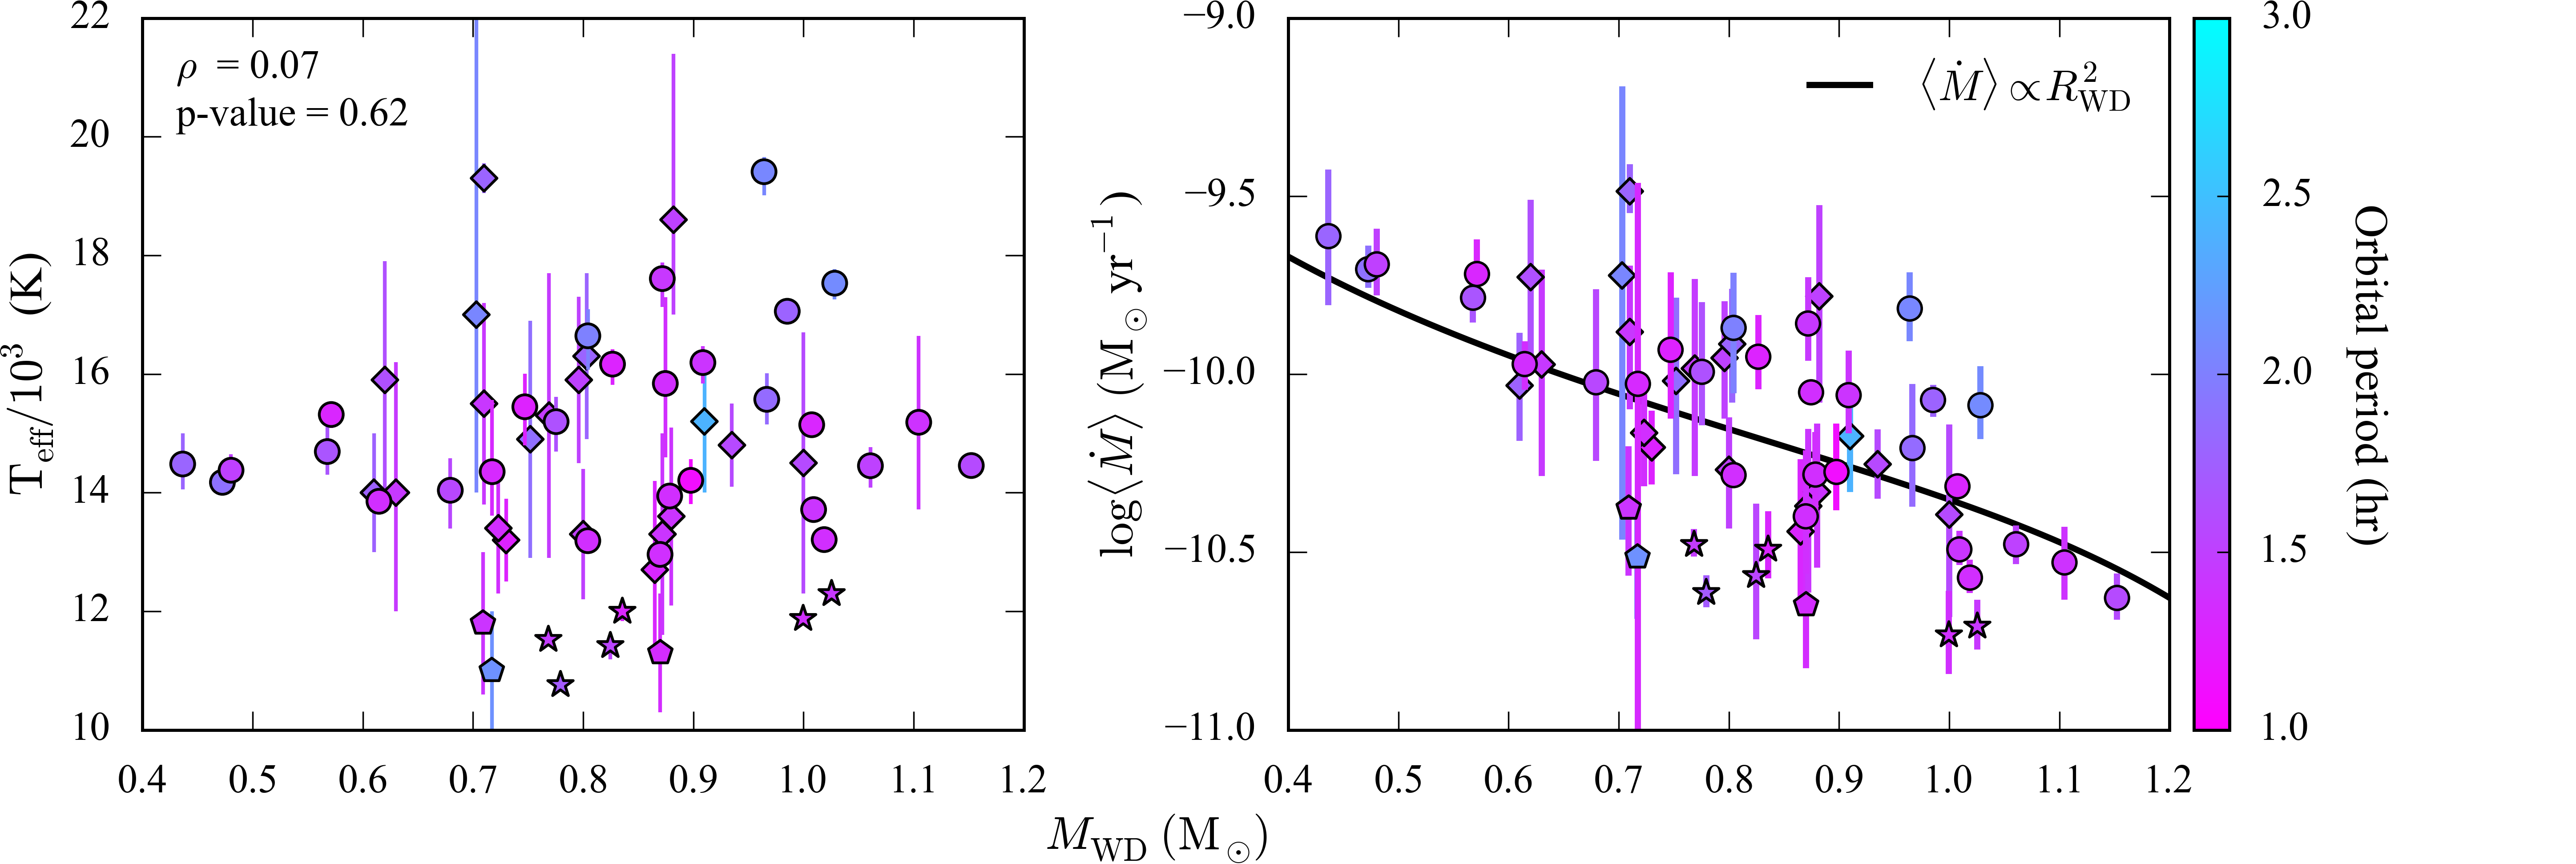
\includegraphics[width=\textwidth]{figures/modelling/pala_2022_fig13.png}
    \caption{Reproduced from \citet{Pala2021}, Figure~13. The subset of modelled systems, with $P < 3{\rm hr}$ are shown. {\bf Circles} and {\bf stars} are pre- and post-period bounce systems derived by \citet{Pala2021}, and {\bf diamonds} and {\bf pentagons} are pre- and post-period bounce systems taken from the literature. {\it Left}: The $T_{\rm eff}$ is plotted against $M_{\rm wd}$, and no correlation can be seen. {\it Right}: $\log<\dot M>$ is plotted against $M_{\rm wd}$, though now the data are correlated along the white dwarf mass-radius relationship assumed by \citet{Pala2021}, $M_{\rm wd} \propto R_{\rm wd}^1.8$. The {\bf black line} shows the rough relationship, and guides the eye.}
    \label{fig:modelling:pala2022 fig13}
\end{figure}


\begin{table}
    \centering
    \caption{The $\dot M$ found using the white dwarf properties for each system with a $\dot M$ measurement from donor properties. Sources are keyed the same as Table~\ref{table:results:mdot modelling}}
    \label{table:results:Mdot from white dwarf parameters}
    \begin{tabular}{llccc}
        \hline
        \textbf{Name} & \textbf{Source} & \textbf{$M_{\rm wd}, M_\odot$} & \textbf{$T_{\rm eff}$, K} & \textbf{$\log (\dot M, M_\odot {\rm yr}^{-1})$} \\
        \hline \hline \\
        ASASSN-14hq      &  W22  & $0.67 \pm 0.01$ & $14800\pm   800$ & $ -9.93 \pm 0.02$ \\
        ASASSN-14kb      &  W22  & $0.74 \pm 0.02$ & $17700\pm  1000$ & $ -9.90 \pm 0.03$ \\
        ASASSN-15pb      &  W22  & $0.72 \pm 0.03$ & $19200\pm  1600$ & $ -9.85 \pm 0.04$ \\
        ASASSN-17fo      &  W22  & $0.85 \pm 0.01$ & $14800\pm   600$ & $-10.03 \pm 0.02$ \\
        AY For           &  W22  & $0.78 \pm 0.02$ & $18200\pm   500$ & $ -9.91 \pm 0.02$ \\
        CSS090102        &  W22  & $0.62 \pm 0.03$ & $14800\pm  1200$ & $ -9.90 \pm 0.04$ \\
        CSS090419        &  W22  & $0.59 \pm 0.08$ & $18200\pm  9000$ & $ -9.79 \pm 0.28$ \\
        CSS090622        &  W22  & $0.67 \pm 0.06$ & $ 9800\pm  1500$ & $-10.11 \pm 0.08$ \\
        MAS0014          &  W22  & $0.86 \pm 0.03$ & $17300\pm  1000$ & $ -9.97 \pm 0.03$ \\
        OGLE82           &  W22  & $0.84 \pm 0.02$ & $18000\pm  4400$ & $ -9.95 \pm 0.12$ \\
        SDSS J0748       &  W22  & $0.80 \pm 0.05$ & $28400\pm  3300$ & $ -9.73 \pm 0.06$ \\
        SDSS J1524       &  W22  & $0.80 \pm 0.04$ & $12500\pm  1100$ & $-10.08 \pm 0.05$ \\
        ASASSN-16kr      &  W20  & $0.95 \pm 0.02$ & $11500\pm   300$ & $-10.19 \pm 0.01$ \\
        ASASSN-17jf      &  W20  & $0.70 \pm 0.03$ & $12020\pm   850$ & $-10.03 \pm 0.04$ \\
        SSSJ1502-3505    &  W20  & $0.76 \pm 0.02$ & $22800\pm  1500$ & $ -9.80 \pm 0.03$ \\
        CSS080623        &  M19  & $0.71 \pm 0.02$ & $15500\pm  1700$ & $ -9.94 \pm 0.05$ \\
        CSS110113        &  M19  & $1.00 \pm 0.05$ & $14500\pm  2200$ & $-10.11 \pm 0.07$ \\
        CTCV 1300-3052   &  M19  & $0.72 \pm 0.02$ & $11000\pm  1000$ & $-10.09 \pm 0.04$ \\
        DV UMa           &  M19  & $1.09 \pm 0.03$ & $17400\pm  1900$ & $-10.07 \pm 0.05$ \\
        GY Cnc           &  M19  & $0.88 \pm 0.02$ & $25900\pm  2300$ & $ -9.81 \pm 0.04$ \\
        IY UMa           &  M19  & $0.96 \pm 0.01$ & $18000\pm  1000$ & $-10.00 \pm 0.02$ \\
        OY Car           &  M19  & $0.88 \pm 0.02$ & $18600\pm  2800$ & $ -9.95 \pm 0.07$ \\
        SDSS 0901        &  M19  & $0.75 \pm 0.02$ & $14900\pm  2000$ & $ -9.98 \pm 0.06$ \\
        SDSS 1006        &  M19  & $0.82 \pm 0.11$ & $16500\pm  2000$ & $ -9.97 \pm 0.08$ \\
        SDSS 1152        &  M19  & $0.62 \pm 0.04$ & $15900\pm  2000$ & $ -9.87 \pm 0.06$ \\
        SDSS 1501        &  M19  & $0.72 \pm 0.02$ & $14900\pm  1000$ & $ -9.96 \pm 0.03$ \\
        SSS100615        &  M19  & $0.88 \pm 0.03$ & $13600\pm  1500$ & $-10.09 \pm 0.05$ \\
        SSS130413        &  M19  & $0.84 \pm 0.03$ & $24000\pm  3000$ & $ -9.82 \pm 0.06$ \\
        V713 Cep         &  M19  & $0.70 \pm 0.02$ & $17000\pm  6000$ & $ -9.89 \pm 0.19$ \\
        Z Cha            &  M19  & $0.80 \pm 0.01$ & $16300\pm  1400$ & $ -9.97 \pm 0.04$ \\
        SDSS J1057+2759  &  M17a & $0.80 \pm 0.02$ & $13300\pm  1100$ & $-10.06 \pm 0.04$ \\
        ASASSN-14ag      &  M17b & $0.63 \pm 0.04$ & $14000\pm  2100$ & $ -9.93 \pm 0.07$ \\
        PHL 1445         &  M15  & $0.73 \pm 0.03$ & $13200\pm   700$ & $-10.02 \pm 0.03$ \\
        \hline
    \end{tabular}
\end{table}

\begin{table}
    \centering
    \caption{Table~\ref{table:results:Mdot from white dwarf parameters}, continued}
    \label{table:results:Mdot from white dwarf parameters cont}
    \begin{tabular}{llccc}
        \hline
        \textbf{Name} & \textbf{Source} & \textbf{$M_{\rm wd}, M_\odot$} & \textbf{$T_{\rm eff}$, K} & \textbf{$\log (\dot M, M_\odot {\rm yr}^{-1})$} \\
        \hline \hline \\
        CTCV J1300-3052  &  S11  & $0.74 \pm 0.01$ & $11100\pm   800$ & $-10.10 \pm 0.03$ \\
        CTCV J2354-4700  &  S11  & $0.94 \pm 0.03$ & $14800\pm   700$ & $-10.08 \pm 0.02$ \\
        SDSS J1152       &  S11  & $0.56 \pm 0.03$ & $12400\pm  1400$ & $ -9.93 \pm 0.06$ \\
        OU Vir           &  S11  & $0.70 \pm 0.01$ & $22300\pm  2100$ & $ -9.77 \pm 0.04$ \\
        % DV UMa           &  S11  & $1.10 \pm 0.02$ & $15500\pm  2400$ & $-10.13 \pm 0.07$ \\
        XZ Eri           &  S11  & $0.77 \pm 0.02$ & $15300\pm  1900$ & $ -9.98 \pm 0.06$ \\
        SDSS J1702        &  S11  & $0.91 \pm 0.03$ & $15200\pm  1200$ & $-10.05 \pm 0.04$ \\
        SDSS J1035        &  S11  & $0.84 \pm 0.01$ & $10000\pm  1100$ & $-10.20 \pm 0.05$ \\
        SDSS J1507        &  S11  & $0.89 \pm 0.01$ & $11300\pm  1000$ & $-10.17 \pm 0.04$ \\
        SDSS J0903        &  S11  & $0.87 \pm 0.01$ & $13300\pm  1700$ & $-10.09 \pm 0.06$ \\
        SDSS J1227        &  S11  & $0.80 \pm 0.02$ & $15900\pm  1400$ & $ -9.98 \pm 0.04$ \\
        SDSS J1433        &  S11  & $0.87 \pm 0.01$ & $12700\pm  1500$ & $-10.11 \pm 0.05$ \\
        SDSS J1502        &  S11  & $0.709\pm0.004$ & $11800\pm  1200$ & $-10.05 \pm 0.04$ \\
        % SDSS J1501        &  S11  & $0.77 \pm 0.03$ & $10800\pm  1500$ & $-10.13 \pm 0.06$ \\
        IP Peg           &  C10  & $1.16 \pm 0.02$ & $12500\pm  2500$ & $-10.24 \pm 0.09$ \\
        \hline
    \end{tabular}
\end{table}







\section{Exploration of the data}
\label{sect:massloss and AML:exploring massloss data}

First, I compare the mass loss rates of the donor inferred from donor properties with the mass loss rates inferred from the white dwarf properties.
Figure~\ref{fig:massloss and AML:compare Mdot from donor and WD} plots the $\dot M$ from each method as a function of period. Note that this figure plots all the white dwarf based $\dot M$, regardless of if they were able to have donor based $\dot M$ found, so not every black point has a corresponding red point.
It is immediately obvious that the white dwarf properties indicate a higher $\dot M$ than the donor properties, and do not closely follow the modelled donor tracks as the CV ages.
Conversely, the donor-derived $\dot M$ closely follows the `optimal' MESA model with gravitational braking amplified by a factor of $2.47$.
Interestingly, the white dwarf properties suggest a much more \textit{consistent} mass loss rate across the CV population, with a tight scatter about $\log (\dot M, M_\odot\ {\rm yr}^{-1}) = \sim -10$ across the full period range. Correlations between the donor-derived $\dot M$ are explored more thoroughly in \S\ref{sect:massloss and AML:mass loss rate correlations}

The white dwarf indicating a higher mass loss rate likely a result of recent dwarf novae (i.e. periods of intense accretion onto the white dwarf), which cause the surface to heat up. After a dwarf nova has subsided, the white dwarf will take hundreds to tens of thousands of years to readjust its temperature to the lower accretion rate, and for that period appear to show a higher accretion rate than is occuring.
Several of the CVs in this sample were identified for eclipse modelling follow-up \textit{explicitly} based on observations of recent outbursts, so it is unsurprising that the white dwarf can indicate $\dot M$ up to an order of magnitude higher than the donor suggests.
As the white dwarf is subject to inflation by these short-term variations and the donor is not, the donor-based method is considered more reliable for the long-term $\dot M$ baseline and hereafter when values of $\dot M$ are used, they are the values derived from the donor properties.
\begin{figure}
    \centering
    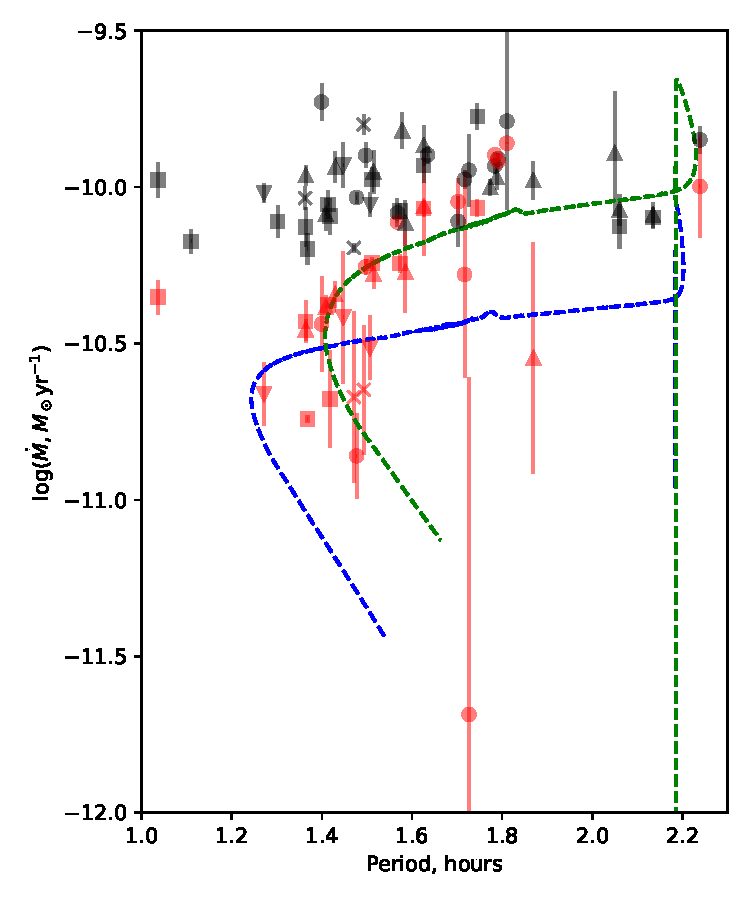
\includegraphics[width=\textwidth]{figures/results/Mdot/compare_mdot_from_donor_vs_wd_vs_period.pdf}
    \caption{Comparing the mass loss rates inferred from the donor properties ({\bf red data}) with those inferred from the white dwarf properties ({\bf black data}). The MESA donor tracks are also plotted; the {\bf blue dashed line} shows the purely gravitational wave driven model, and the {\bf green dashed line} shows the model with gravitational braking amplified by a factor of $2.47$. The symbols denote the source of the data, The {\bf circles} are the systems from Chapter~\ref{chpt:results:characterisation of 12 new CVs}, {\bf upright triangles} are data from \citet{McAllister2019}, {\bf squares} are from \citet{Savoury2011}, and the {\bf inverted triangle} is the supplementary system from \citet{mcallister2017b}.}
    \label{fig:massloss and AML:compare Mdot from donor and WD}
\end{figure}

\newpage
\subsection{Mass loss rate correlations}
\label{sect:massloss and AML:mass loss rate correlations}

Recall from the discussion in \S\ref{sect:introduction:magnetic braking} that, if the missing AML from CV models is rooted in residual magnetic braking, \textit{and these prescriptions for magnetism are accurate}, we would expect to see a correlation between $M_{\rm donor}$ and $\dot M$, and see no such correlation with $M_{\rm wd}$.
This is because both magnetic braking prescriptions considered are dependent on the Rossby number, a function of the rotational period, which itself is a function of donor mass for short period CVs. Note that the allowed mass range of the method used here forces us to omit period bouncer systems.
If, however, the eCAML model is the source of the missing AML is the white dwarf's ejecta carrying momentum with it from the system (refer to \S\ref{sect:introduction:CAML}), we would expect a correlation between $M_{\rm wd}$ and $\dot M$, as the white dwarf dominates the total mass in short period CVs.
Of course, the two sources of extra AML are not mutually exclusive and may co-exist.

To probe for these correlations the $\chi^2$ test is insufficient, since both axes have significant uncertainty. The orthogonal distance between the line and data is again minimised, similar to the previous section.
Also, in this section I use Pearson correlation coefficients and their associated $p$ values; these are computed based on the \textit{means} of the data, and do not consider the uncertainty in the measurements.
Whilst not technically valid, these values serve as a useful rough guide and are often easily corroborated by inspection of the relevant plots\footnote{Pearson correlation coefficients range from $-1$ (perfect negative correlation), to $+1$ (perfect positive correlation), with 0 indicating no correlation between the data. The $p$ value is the probability of the null hypothesis, i.e. that the data are uncorrelated, and values of $p < 0.05$ are generally accepted to indicate confidence.}.

Figure~\ref{fig:massloss and AML:white dwarf mass vs Mdot fit} shows the data for $\dot M(M_{\rm wd})$, and Figure~\ref{fig:massloss and AML:donor mass vs Mdot fit} shows $\dot M(M_{\rm donor})$.
The correlation between $M_{\rm wd}$ and $\dot M$, is reasonably confident; ignoring errors, these data have a Pearson rank correlation coefficient of $-0.502$, with a $p$ value of $0.012$, indicating a mild correlation with a high likelihood. Fitting a straight line to these data confirms this, finding a best-fit gradient that is $4.5\sigma$ from the null-hypothesis of 0.
However, no correlation is found between $\dot M$ and $M_{\rm donor}$. These data have a Pearson coefficient of $0.089$ with a $p$ value of $0.68$, suggestive of no correlation.

% \todo{Why? I can't think of anything hugely convincing. The period and mass are closely linked in the models, so I would have expected the close agreement to translate pretty well, maybe with larger errorbars.}
Figure~\ref{fig:massloss and AML:compare Mdot from donor and WD} shows a reasonably tight agreement between the $\dot M$ and period, and we might expect to see this reflected in the donor mass, given the strong dependence of $M_{\rm donor}$ on period, but the agreement is far more ambiguous with many data lying between the two model tracks, rather than lying directly on the `optimal' model. This is likely an artifact of the scatter about the models in Figure~\ref{fig:12 new cvs:donor model with eclipsers plotted}, as the mass-period relationship is synonymous with the mass-period relationship, so the scatter in Figure~\ref{fig:12 new cvs:donor model with eclipsers plotted} propagates forward.\todo{This probably doesn't sound good. Think some more, or at least rework the sentence.}

Based on these results, it appears unlikely that residual magnetic braking (in the forms given in \S\ref{sect:introduction:magnetic braking}) is responsible for the excess AML in CVs, but still possible that the drag imposed by nova material is the cause.
However, there are a few factors to consider when deciding how convincing these findings are.
The sample size is still small, only 25 systems, and the uncertainty in these measurements is significant.
More importantly, the parameter space in the $0.12 M_\odot < M_{\rm donor} < 0.20 M_\odot$ is sparsely populated, and has particularly large uncertainty. This makes the search for correlation dominated by data in the narrow range of $0.08 M_\odot < M_{\rm donor} < 0.12 M_\odot$, and thus less robust; gathering more data for short period CVs with higher $M_{\rm donor}$ may reveal a correlation between donor mass and mass loss rate.
Also, this lack of correlation could be a consequence of even the amplified `optimal' model $\dot M$ not varying by much across the available mass range, a problem that will similarly be solved by expanding the available sample.
In addition, there may be a problem with systematic error -- it may that this sample is biased towards CVs with more excess AML. Systems with higher AML rates would be more inflated and thus less likely to be smaller than the Brown relation suggests for a zero-$\dot M$ star, omitting them from the sample.
Finally, as mentioned in \S\ref{sect:modelling:donor mass loss rates}, a significant source of unreliability is likely to be the mass-radius relationship used to calibrate the donor models. A more robust understanding of the low-mass main sequence mass-radius relation is crucial to a more confident re-analysis of these results.

\begin{figure}
    \centering
    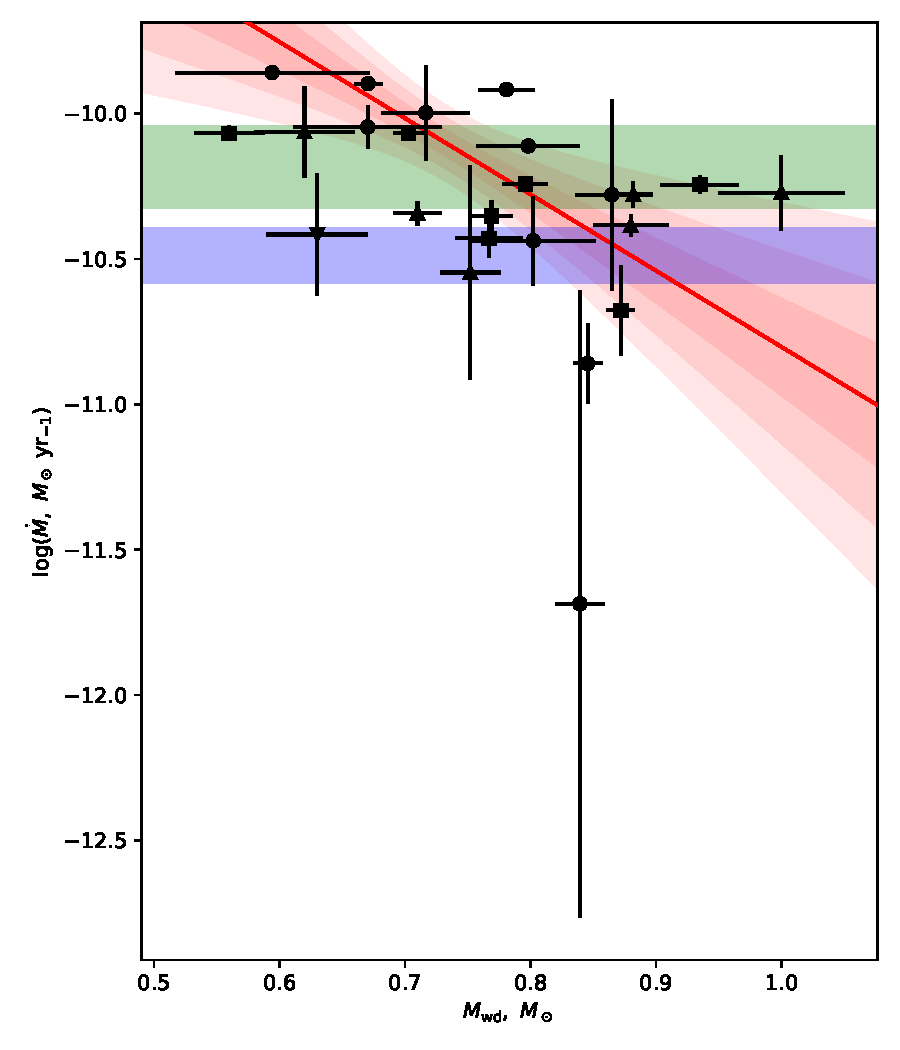
\includegraphics[width=\textwidth]{figures/results/Mdot/Mwd_Mdot.pdf}
    \caption{Showing the correlation between the white dwarf mass and mass loss rate. The {\bf black circles} are the systems from Chapter~\ref{chpt:results:characterisation of 12 new CVs}, {\bf gold upright triangles} are data from \citet{McAllister2019}, {\bf grey squares} are from \citet{Savoury2011}, and the {\bf brown inverted triangle} is the supplementary system from \citet{mcallister2017b}. The range of mass loss rates predicted by the `standard' and `optimal' MESA CV models are shown as the {\bf blue shaded region} and {\bf green shaded region}, respectively. The {\bf red line} shows the best fit to the data, with the {\bf shaded red region} showing the coverage of the uncertainty in the line parameters. The darkest region is $1\sigma$, the middle region is $2\sigma$, and the lightest region shows $3\sigma$, and the {\rm brown line} is the initial guess for fitting. The best fit line has the form $\log ( \dot M,\ M_\odot\ {\rm yr}^{-1}) = (-2.62 \pm 0.60) (M_{\rm wd}, M_\odot) - (8.18 \pm 0.44)$.}
    \label{fig:massloss and AML:white dwarf mass vs Mdot fit}
\end{figure}
\begin{figure}
    \centering
    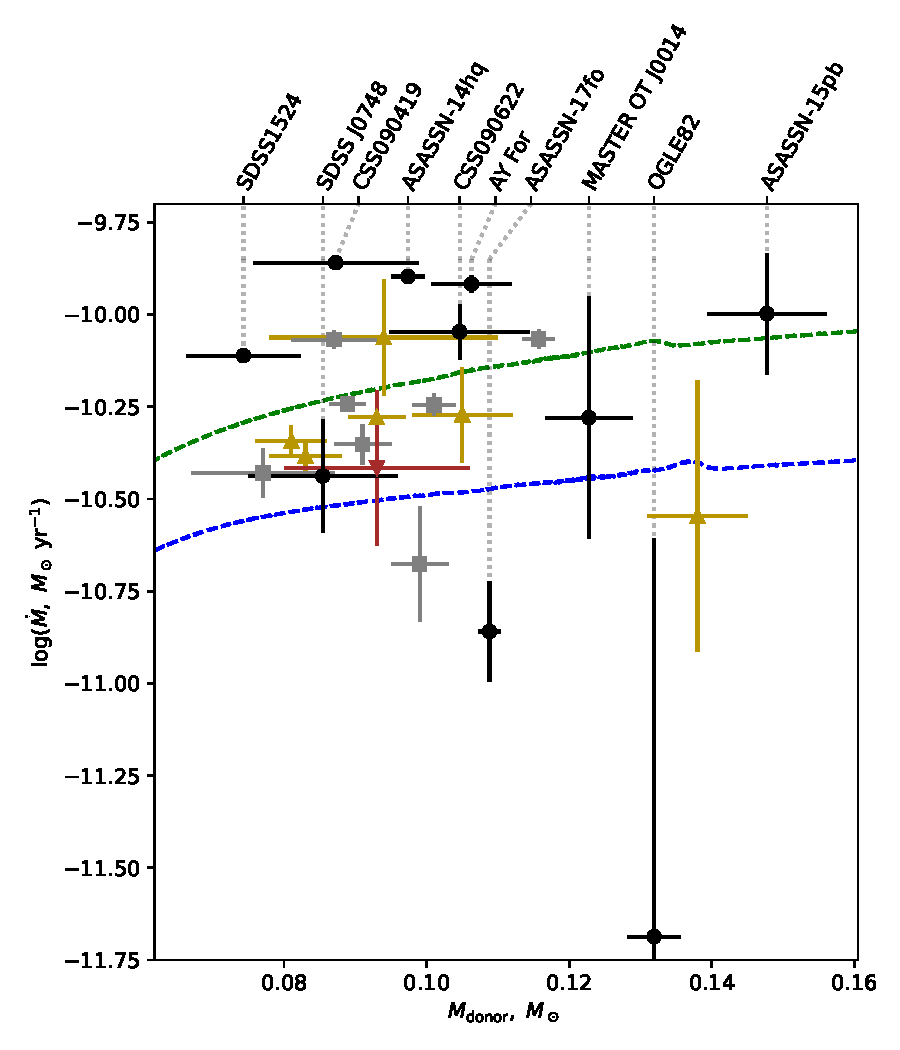
\includegraphics[width=\textwidth]{figures/results/Mdot/Mr_Mdot_nofit.pdf}
    \caption{Showing the donor masses and mass loss rates. Observations are styled similarly to Figure~\ref{fig:massloss and AML:white dwarf mass vs Mdot fit}. The {\bf dashed blue line} shows the value predicted by the `standard' MESA CV model, and the {\bf dashed green line} is the `optimal' MESA CV track.}
    \label{fig:massloss and AML:donor mass vs Mdot fit}
\end{figure}



\newpage
\subsection{Measured angular momentum loss}

It is possible to more directly probe the AML of the CVs -- Equation~\ref{eqn:modelling:Jdot from Mdot} shows how the AML can be calculated from $M_{\rm wd},\ M_{\rm donor},\ \dot M$, and $a$.
Figures~\ref{fig:massloss and AML:donor mass vs Jdot fit}~and~\ref{fig:massloss and AML:white dwarf mass vs Jdot fit} show the best-fit to the $\dot J$ \textit{excess}, $\dot J_{\rm ex}$, which has had the $\dot J_{\rm GR}$ subtracted.

The $M_{\rm wd}$ and $\dot J_{\rm ex}$ data appear to be loosely correlated, with a Pearson correlation of $-0.514$ and a p-value of $0.010$. Fitting a straight line to the data finds $(\dot J_{\rm obs} - \dot J_{\rm MESA}), J = (-8.3\pm1.6) \times 10^{27}(M_{\rm wd}, M_\odot) + (6.9\pm1.3)\times10^{27}$.
However, similarly to the $\log (\dot M)$ data, there is no sign of correlation for $M_{\rm donor}$. The $\dot J_{\rm ex}$ data have a correlation coefficient of $0.032$, and a p-value of $0.884$, strongly indicating that the data are uncorrelated.
% The lack of correlation here with $M_{\rm donor}$ is strange when we consider the tight agreement with models seen in Figure~\ref{fig:massloss and AML:compare Mdot from donor and WD}.
\todo{You forgot to cut the low mass stars! Fix that.}

\begin{figure}
    \centering
    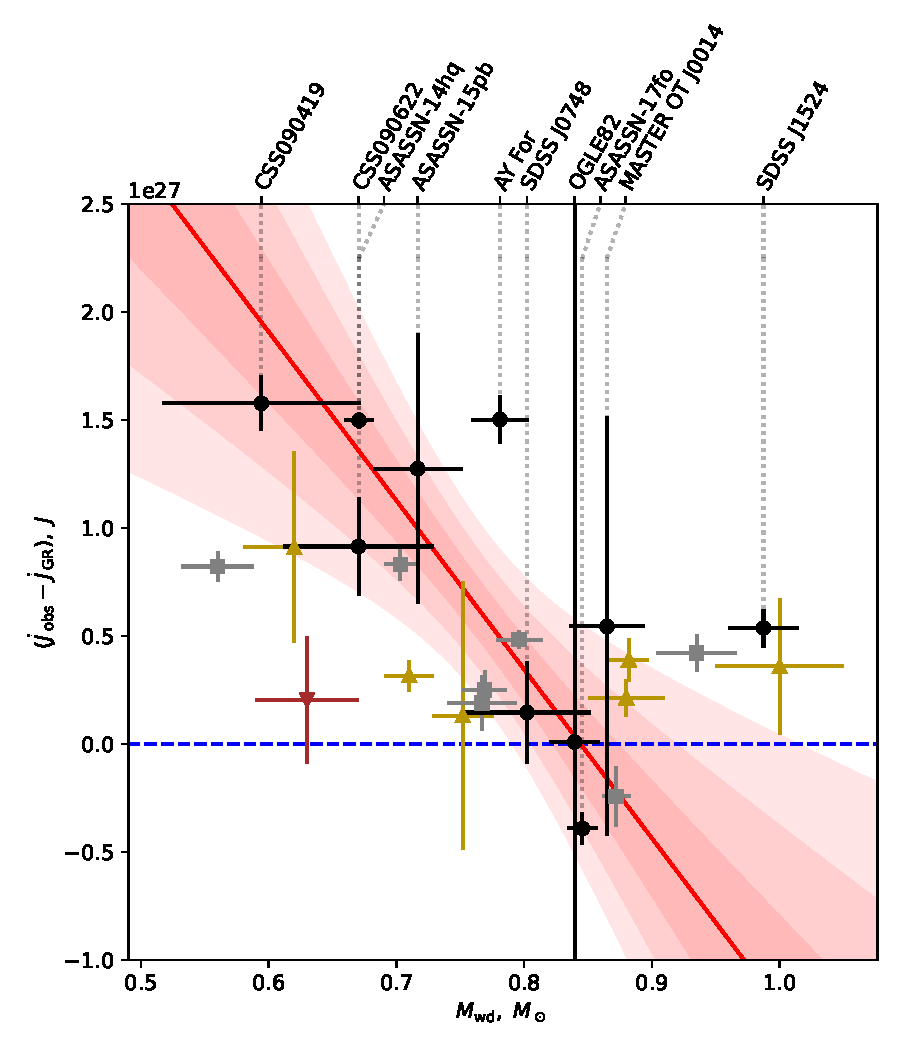
\includegraphics[width=\textwidth]{figures/results/Mdot/Mwd_Jdot_ex.pdf}
    \caption{Showing the correlation between the white dwarf mass and angular momentum loss rate, $\dot J$. Observations are keyed similarly to Figure~\ref{fig:massloss and AML:white dwarf mass vs Mdot fit}, and the best fit line has the form $(\dot J_{\rm obs} - \dot J_{\rm MESA}), J = (-8.3\pm1.6) \times 10^{27}(M_{\rm wd}, M_\odot) + (6.9\pm1.3)\times10^{27}$. Note that the datum with vertical errors spanning the full height of the plot extend by approximately an order of magnitude in each direction, but are truncated for clarity.}
    \label{fig:massloss and AML:white dwarf mass vs Jdot fit}
\end{figure}
\begin{figure}
    \centering
    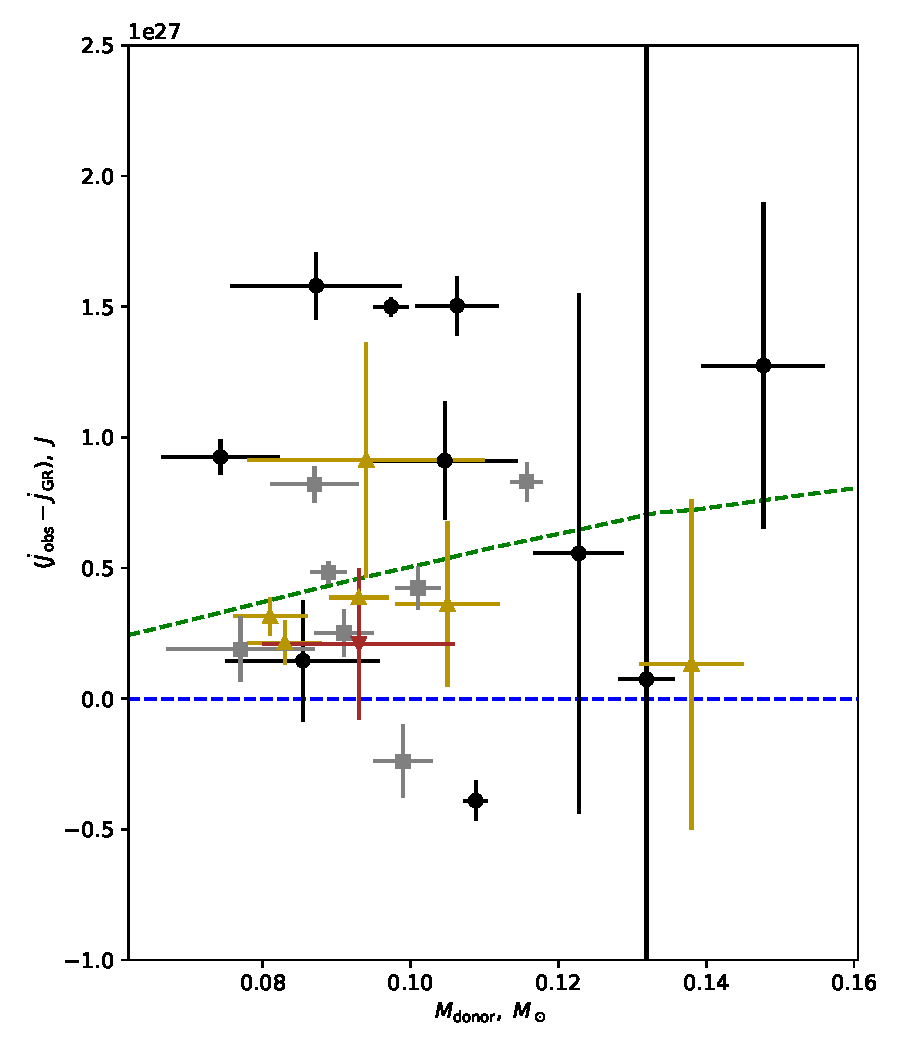
\includegraphics[width=\textwidth]{figures/results/Mdot/Mr_Jdot_nofit.pdf}
    \caption{Showing the correlation between the donor mass and angular momentum loss rate, $\dot J$. Observations are keyed similarly to Figure~\ref{fig:massloss and AML:white dwarf mass vs Mdot fit}, though here the {\bf dashed blue line} shows perfect agreement between observations and gravitational angular momentum loss. The {\bf dashed green line} shows the $2.47\times$ donor track. Note that the datum with vertical errors spanning the full height of the plot extend by approximately an order of magnitude in each direction, but are truncated for clarity.}
    \label{fig:massloss and AML:donor mass vs Jdot fit}
\end{figure}


Three possibilities for the form of excess AML were suggested in \S\ref{sect:12 new cvs:period excess}: the excess AML also declines in strength but more slowly than gravitational losses; excess AML is roughly constant across the range of $M_{\rm donor}$ or $M_{\rm donor}$; or excess AML increases in strength towards lower $M_{\rm donor}$ or $M_{\rm wd}$.
We can now see that the excess AML appears to increase in strength towards lower $M_{\rm wd}$, and is uncorrelated with $M_{\rm donor}$.

Recall from \S\ref{sect:introduction:CAML} that under eCAML, the efficiency parameter $\nu$ is given by $C/M_{\rm wd}$, and typical values of $C$ are roughly chosen to be $0.3 - 0.4$ to reproduce the observed CV population distribution.
\begin{gather}
    \frac{\dot J_{CAML}}{J} = \nu \frac{\dot M_{\rm donor}}{M_{\rm donor}} \label{eqn:ecaml general} \\
    \frac{\dot J_{CAML}}{J} = C \frac{\dot M_{\rm donor}}{M_{\rm donor} M_{\rm wd}}
\end{gather}
$C$ can now be fit to data, again minimising the orthogonal distance, though this fit is limited to the subset of the subset of observations for which $\dot M$ could be determined.
Doing so finds a best-fit $C =$\todo{Think hard about this analysis!} with impressively good agreement between the model and data, shown in Figure~\ref{fig:massloss and AML:calibrating ecaml relationship}. This value of $C$ is also remarkably close to that estimated by \citet{Schreiber2016}. \todo{This is the wrong one! I need the one with no y-intercept.}
\begin{figure}
    \centering
    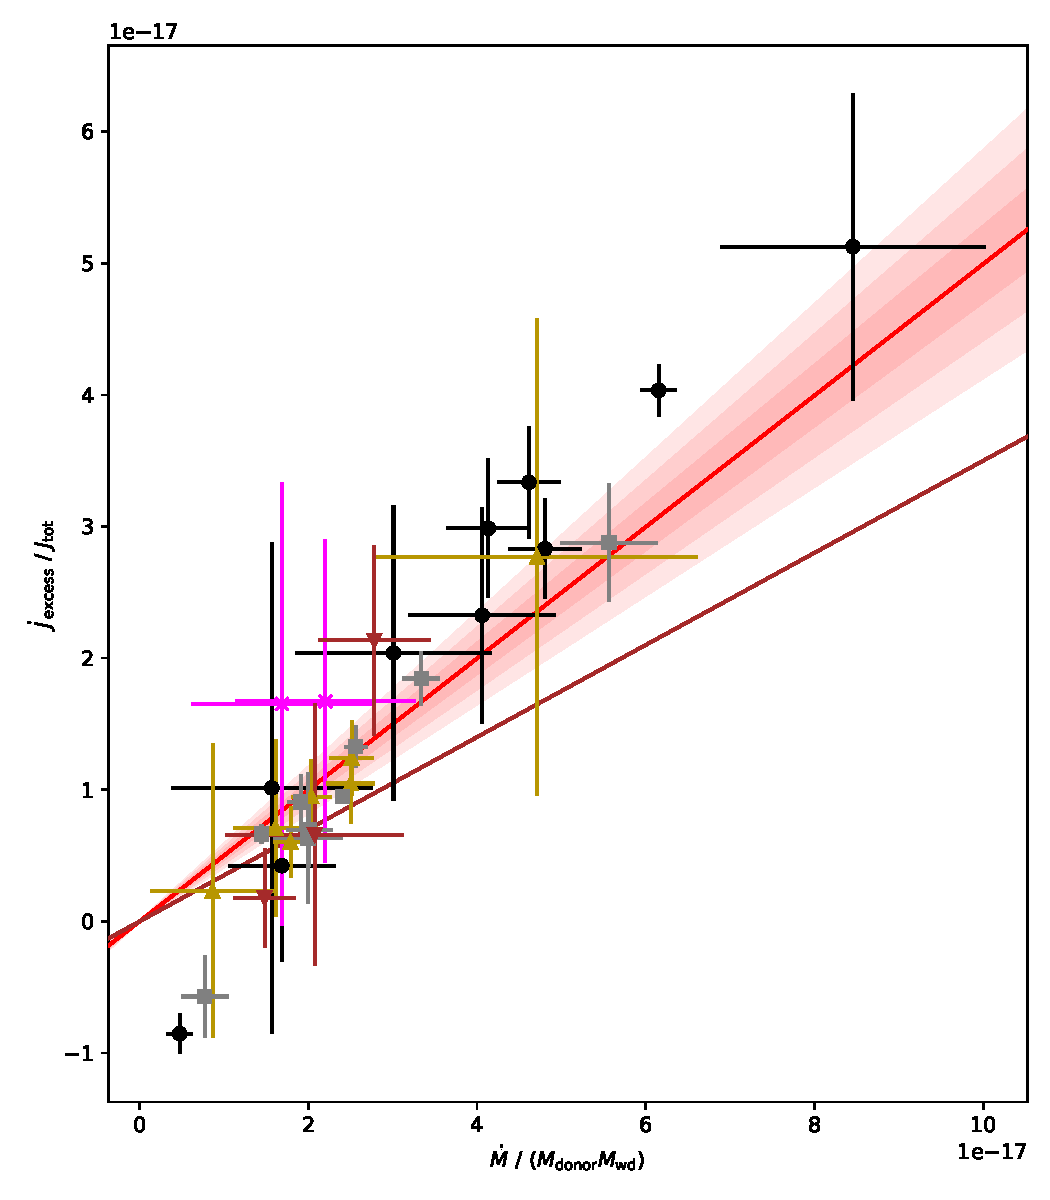
\includegraphics[width=\textwidth]{figures/results/Mdot/eCAML_nu_no_intercept_fit.pdf}
    \caption{DO THIS CAPTION}
    \label{fig:massloss and AML:calibrating ecaml relationship}
\end{figure}

As a final test of eCAML, the stability plot given in Figure~\ref{fig:introduction:Schreiber 2016 figure 2} can be augmented to include the new CVs of this work, and the best-fit value of $\nu$.\todo{Fix the label!}
This is shown in Figure~\ref{fig:massloss and AML:calibrated eCAML}, from which we can see that no low $M_{\rm donor}$ CVs exist outside the stability region demanded by the newly calibrated eCAML.
\begin{figure}
    \centering
    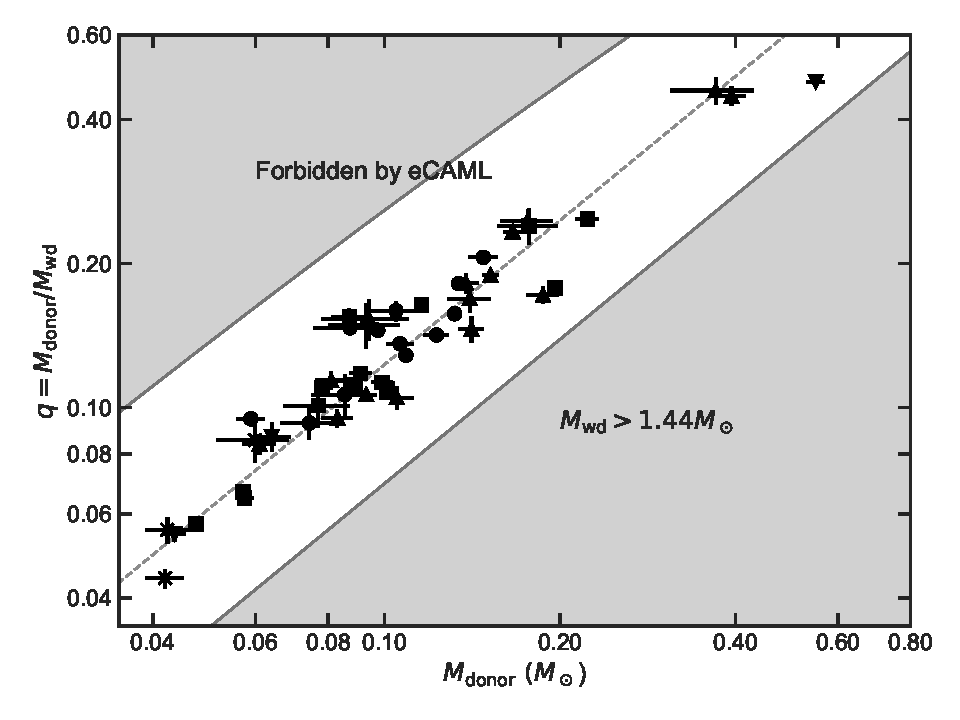
\includegraphics[width=\textwidth]{figures/results/Mdot/ecaml_nointercept.pdf}
    \caption{Showing the distribution of eclipse modelled, low $M_{\rm donor}$ CVs compared to the region of stability demanded by eCAML. The {\bf shaded grey regions} are forbidden, either because the white dwarf exceeds the Chandrasekhar limit (lower region), or because mass transfer becomes dynamically unstable (upper region). The {\bf dashed line} shows the mass ratio that a CV would have with $M_{\rm wd} = 0.81 M_\odot$. Data symbology is similar to Figure~\ref{fig:massloss and AML:donor model with eclipsers plotted}}
    \label{fig:massloss and AML:calibrated eCAML}
\end{figure}
These findings underline the success of eCAML in describing CV evolution, but must still be treated with caution. It cannot be ignored that whilst this form of $\nu$ is loosely physically motivated, a less empirical model is highly desirable.
Further, the data clearly suggest that $\frac{\dot J_{CAML}}{J} \neq 0$ at $\dot M = 0$, in direct contradiction with the original formulation. \todo{Talk to Stu about this when he's back. I reckon some algebra is needed to re-derive the stability criterion to allow for this... But it's not physical! How could CAML inhibit AML???}

Further work is needed to grow the population of eclipse modelled low-$M_{\rm donor}$ CVs and improve these statistics, and continued eclipse modelling targeting short period CVs will be valuable to determining the probable source of excess AML.
Specific effort should be targeted towards confident characterisation of CVs at higher $M_{\rm donor}$ of $\sim0.15$, where existing data have large error bars. The clustering of confident data at lower masses leaves the current sample prone to poor extrapolation beyond $\sim 0.11 M_\odot$.
However, lending credence to these results is the consistency with findings of \citet{Pala2021}, who used the white dwarf properties to arrive at a similar conclusion.

\todo{Augment MESA to include my new AML prescription, and run it?}